\documentclass[conference]{IEEEtran}
\IEEEoverridecommandlockouts

\usepackage{amsmath,amssymb,amsfonts}
\usepackage{algorithmic}
\usepackage{graphicx}
\usepackage{textcomp}
\usepackage{xcolor}
\usepackage{minted}
\usepackage{hyperref}

\usepackage[utf8]{inputenc}
\usepackage[T1]{fontenc}
\usepackage[english]{babel}
\usepackage{ethiop}

\graphicspath{ {charts/} }

\usepackage{biblatex}
\addbibresource{references.bib}
\def\BibTeX{{\rm B\kern-.05em{\sc i\kern-.025em b}\kern-.08em
    T\kern-.1667em\lower.7ex\hbox{E}\kern-.125em}}

\begin{document}

\selectlanguage{english}
\title{Amharic language letter frequency distribution\\}
\author{\IEEEauthorblockN{Samson Endale Mergissa}
\IEEEauthorblockA{\textit{Crypo analysis (IP team)} \\
\textit{Information Network Security Agency}\\
Addis Ababa, Ethiopia \\
samson.endale@insa.gov.et, 4sam21@gmail.com}
}

\maketitle

\begin{abstract}
One of the first and famous attacks on classical cryptographic algorithms is frequency analysis. It requires the letter frequency of the given language available to implement this attack. Even if an Amharic text is encrypted with a simple mono-alphabetic substitution, we couldn't break the cipher with frequency analysis because the Amharic language never been analyzed to learn the letter frequency distribution. I have tried to address this problem by collecting and analyzing a relatively large dataset of Amharic texts. This analysis and findings are done for the first time for this language and I have uncovered fascinating statistical distributions of the language.
\end{abstract}

\begin{IEEEkeywords}
Amharic, frequency distribution, cryptanalysis  
\end{IEEEkeywords}

\section{Introduction}

\subsection{The Amharic language (\foreignlanguage{ethiop}{'amAre~nA})}

Amharic is a Semitic language and the national language of Ethiopia (\foreignlanguage{ethiop}{'iteyo.peyA}). The majority of the 25 million or so speakers of Amharic can be found in Ethiopia\cite{csa_census_report}, but there are also speakers in a number of other countries, particularly Eritrea , Canada, the USA and Sweden. Amharic is written with a version of the Ge'ez script known as \foreignlanguage{ethiop}{fidale} (Fidel)\cite{omniglot}. Amharic is the second-most commonly spoken Semitic language in the world, after Arabic. Amharic is written left-to-right using a system that grew out of the Ge'ez script, called, in Ethiopian Semitic languages, Fidäl (\foreignlanguage{ethiop}{fidale}, "writing system", "letter", or "character" or abugida (\foreignlanguage{ethiop}{'abugidA} from the first four symbols, which gave rise to the modern linguistic term abugida. It has been the working language of courts, language of trade and everyday communications, the military, and the Ethiopian Orthodox Tewahedo Church since the late 12th century and remains the official language of Ethiopia today\cite{lingua_franca}. Most of the Ethiopian Jewish communities in Ethiopia and Israel speak Amharic. In Washington DC, Amharic became one of the six non-English languages in the Language Access Act of 2004, which allows government services and education in Amharic. Furthermore, Amharic is considered a holy language by the Rastafari religion and is widely used among its followers worldwide\cite{dc_language_access_act}. It is the most widely spoken language in the Horn of Africa. The Amharic script is an abugida, and the graphemes of the Amharic writing system are called fidel. Each character represents a consonant+vowel sequence, but the basic shape of each character is determined by the consonant, which is modified for the vowel. This is because these fidel originally represented distinct sounds, but phonological changes merged them. The citation form for each series is the consonant+ä form, i.e. the first column of the fidel. The Amharic script is included in Unicode, and glyphs are included in fonts available with major operating systems\cite{amharic_major_languages}.

\subsection{Frequency analysis}
Among so many cryptanalytic techniques, frequency analysis or frequency count is the most basic one other than brute-force, threat, blackmail, torture, and bribery. The frequency analysis is, in fact, the anatomy of a language. According to a book “Trattati in cifra” published in 1470 and written by Leone Battista Alberti, who is known as “Father of Western Cryptology”, the aspect of cryptanalysis using frequency analysis can be traced back to Al-Kindi, who is “The Philosopher of the Arabs” and author of 290 books on medicine, astronomy, mathematics, linguistics, and music. In 1987, the Arabic scientist Al-Kindi’s treatise was discovered in the Sulaimaniyyah Ottoman Archive in Istanbul and entitled “A Manuscript on Deciphering Cryptographic Message”. It is believed that this manuscript is the first ever known oldest description of cryptanalysis by frequency analysis\cite{decrypting_english_enhanced}.

\subsection{Other applications}
Knowing the frequency distribution is essential for developing optimal encoding schemes for communication mechanism like Telegraph by Morse code. To increase the speed of the communication, the code was designed so that the length of each character in Morse is approximately inverse to its frequency of occurrence in English. Thus the most common letter in English, the letter "E", has the shortest code, a single dot\cite{morse_code}.

Additionally, this analysis is essential for developing a keyboard layout with an efficient hand movement. Letter frequencies had a strong effect on the design of some keyboard layouts. The most frequent letters are on the bottom row of the Blickensderfer typewriter, and the home row of the Dvorak Simplified Keyboard\cite{bbc_qwerty}\cite{qwerty_review}. 

Furthermore, aforementioned also heavily contribute to the field of optical character recognition and in linguistics.

\section{Background}

For almost a thousand years, from 500 CE to 1400 CE, the cryptology of Western civilization stagnated. The systems used were extremely simple and more or less derivations of substitution ciphers and steganography. However the Arabs were the first to discover the importance of cryptanalysis in the 9th century CE. Till this time only cryptography existed and of any science of cryptanalysis there was nothing. Cryptanalysis is the science of unscrambling a message without the knowledge of the key and is based on finding weaknesses in encryption methods in order to break them. The Arabs had the best conditions for inventing cryptanalysis because they had reached a high level in several disciplines, including mathematics, statistics and linguistics. Theological schools were established where the contents of the Koran were studied in detail. Theologians tried to extract a chronological order of the numerous revelations and therefore they counted the frequency of specific words in every single revelation because some words arose earlier in comparison to other words. They continued to examine the scriptures phonetically and at the level of single letters and found out, that some letters occur much more frequently than other ones and which letters go or do not go together. They realized the rarest letters in Arabic and the most common letters: the letters 'a' and 'l' are the most common in Arabic, whereas the letter 'j' appears only a tenth as frequency. This apparently innocuous observation would lead to the first great breakthrough in cryptanalysis, namely frequency analysis. It is unknown who first realized that the variation in the frequencies of letters could be exploited in order to break ciphers, but the earliest known description comes from the 9th century scientist Abū-Yūsuf Ya’qūb ibn Ishāq al-Kindī. Al-Kindi has written about 290 books on medicine, astronomy, mathematics, linguistics and music. He also is the author of 'A Manuscript on Deciphering Cryptographic Messages'. It contains detailed discussions on statistics, Arabic phonetics and Arabic syntax and describes the system of cryptanalysis in two short paragraphs: "\textit{One way to solve an encrypted message, if we know its language, is to find a different plaintext of the same language long enough to fill one sheet or so, and then we count the occurrences of each letter. We call the most frequently occurring letter the 'first', the next most occurring letter the 'second' the following most occurring letter the 'third', and so on, until we account for all the different letters in the plaintext sample. Then we look at the ciphertext we want to solve and we also classify its symbols. We find the most occurring symbol and change it to the form of the 'first' letter of the plaintext sample, the next most common symbol is changed to the form of the 'second' letter, and the following most common symbol is changed to the form of the 'third' letter, and so on, until we account for all symbols of the cryptogram we want to solve}" \cite{frequency_analysis}.

\section{Methodology}

\subsection{Data Gathering}
The first route I took was to collect various religious texts. I successfully manage to find more than 800,000 characters suitable for analyzing. I also tried to gather some Amharic fictions, the constitution, government regulations,  and government reports.

The second place I look for gathering the document was around newspapers which publish a soft-copy on their site. It was a good lead with few newspapers but most of the publisher upload the scanned version of the printed newspaper or the encoding was very bogus and I couldn't extract the Amharic letters.

Lastly, I was googling for Amharic documents by hand which was the least efficient way of tackling the problem. At first, I was looking for a search engine with a regular expression support to search for a document containing the Ethiopic Unicode block which is between 0x1200 to 0x1347. However, most of the search engines lack this functionality which was discouraging. After a lot of effort, I found a more effective method. 

Analyzing the already available data, I found out a glimpse of the frequency distribution of the language with a fewer dataset. It happens to be "\foreignlanguage{ethiop}{n}" is the most frequent character from the religious texts. The letter "\foreignlanguage{ethiop}{n}" most likely will occur at least once in any Amharic document. This was an alternative for filtering am Amharic documents on the web. So I start searching for \texttt{\textbf{"allintext:\foreignlanguage{ethiop}{n} filetype:pdf"}} on Google and the number of the result was promising. Thus I was using as a result of an “Amharic language frequency distribution” of a smaller dataset to gather a larger dataset for “Amharic language frequency distribution”. This method help to gather a lot of random documents which is good for diversifying the dataset but I started to notice a few obstacles.

Most of the documents I found were not larger than 5 pages and I noticed some of the documents were Tigrigna, Ge`ez or some other Ethiopian language which use the Ge’ez script. So I start looking for a better method to query the search engines. At last, I fined tuned my search query to \texttt{\textbf{"allintext:\foreignlanguage{ethiop}{mAwe^CA} filetype:pdf"}}. I noticed word \foreignlanguage{ethiop}{mAwe^CA} usually occurs more frequently in long Amharic documents through observation and it also makes the document more likely an Amharic.

I was also was trying to write a web crawler to index \url{https://am.wikipedia.org} but I dismiss it because like most sites, the layout of the website was a static and repeated in every page. I didn’t want to “poison” my dataset with a "wrong" frequency.

\subsection{Data preparation and clean up}
Before analyzing the PDF format files, I wanted to make sure there was no duplication in the files. I first run \texttt{\textbf{“sha256sum”}} command in a Linux terminal and pipeline the output to \texttt{\textbf{“sort”}}. 

\inputminted{bash}{codes/sha256-sort.sh}

There were some duplicates. Therefore I used a tool called \texttt{\textbf{“fdupes”}} to locate and delete duplicated files.

\mint{bash}{\$ fdupes -d *}

Second I converted all of the PDF files to a plain text using a tool called \texttt{\textbf{“pdftotext”}} because plain text files are easier to process than a PDF format. Lastly, I combined the text files into a giant plain file to shave it to my own analyzer program. The combined text contains 2,245,892 lines,  6,150,197 words and 75,143,429 letters. But I later found out only 17.2 million of the letters were a properly encoded Amharic Unicode characters.

\subsection{Analysis}
The analysis was a straightforward process. I wrote a python program which opens the documents and counts the various frequencies and dumps the result into a CSV file.

\section{Data and Results}

\subsection{Monogram frequency}
Monogram frequency counts are most effective on substitution type ciphers such as the caesar cipher, substitution cipher, polybius square etc. It works because any natural language text follows a very specific frequency distribution, which is not masked by substitution ciphers\cite{text_characterisation}.

\selectlanguage{ethiop}
\begin{table}[h!]
    \begin{center}
        \begin{tabular}{|| r | l | r | r ||}
            \hline
            \foreignlanguage{english}{Rank} & 
            \foreignlanguage{english}{Character} &
            \foreignlanguage{english}{Count} & 
            \foreignlanguage{english}{Percentage} \\
            \hline
            \hline
            1 & n & 738643 & 4.28079 \\
            2 & t & 680710 & 3.94504 \\
            3 & ya & 638802 & 3.70216 \\
            4 & ba & 566363 & 3.28234 \\
            5 & ma & 556450 & 3.22489 \\
            6 & r & 455960 & 2.64251 \\
            7 & w & 436064 & 2.5272 \\
            8 & ta & 427311 & 2.47647 \\
            9 & s & 387069 & 2.24325 \\
            10 & nA & 347901 & 2.01625 \\
            11 & yA & 331325 & 1.92018 \\
            12 & m & 321078 & 1.8608 \\
            13 & 'e & 301741 & 1.74873 \\
            14 & : & 294046 & 1.70413 \\
            15 & 'a & 287540 & 1.66643 \\
            16 & y & 273357 & 1.58423 \\
            17 & ^c & 271122 & 1.57128 \\
            18 & g & 269841 & 1.56386 \\
            19 & ga & 265020 & 1.53592 \\
            20 & ka & 258721 & 1.49941 \\
            21 & ra & 251049 & 1.45495 \\
            22 & mA & 245490 & 1.42273 \\
            23 & l & 244525 & 1.41714  \\
            \hline
        \end{tabular}
    
        \selectlanguage{english}
        \caption{Top 23 - Monogram frequency}
        \label{table:1}
    \end{center}
\end{table}

\selectlanguage{english}
\begin{figure}[H]
    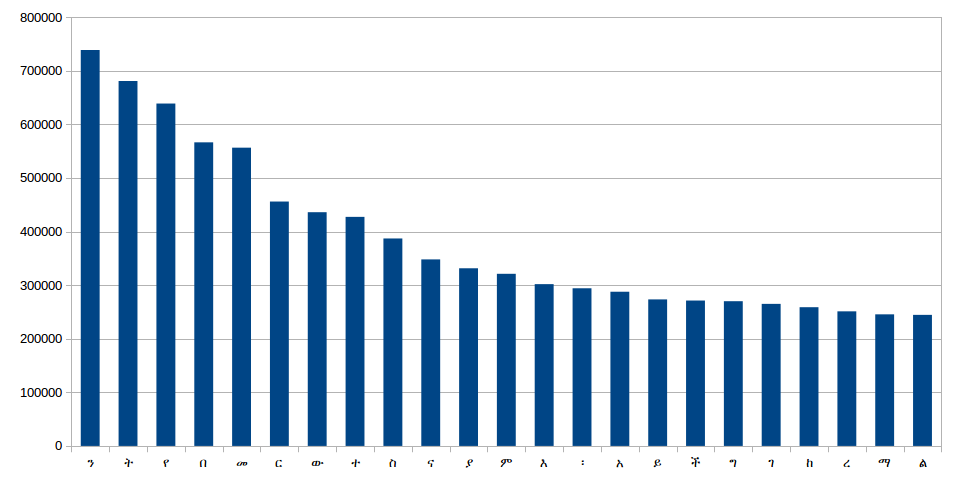
\includegraphics[width=0.48\textwidth]{fig_top23_letters}
    \centering
    \caption{Top 23 - Monogram frequency}
    \label{fig:mesh1}
\end{figure}

\subsection{Bigram frequency}
Bigram counts maintain the same principle as monogram counts, but instead of counting occurrences of single characters, bigram counts count the frequency of pairs of characters\cite{text_characterisation}.

\selectlanguage{ethiop}
\begin{table}[H]
    \begin{center}
        \begin{tabular}{|| r | l | r || r | l | r ||}
        \hline
        \foreignlanguage{english}{ } &
        \foreignlanguage{english}{Character} & 
        \foreignlanguage{english}{Count} & 
        \foreignlanguage{english}{ } &
        \foreignlanguage{english}{Character} &
        \foreignlanguage{english}{Count} \\
        \hline
        \hline
            1 & 'ene & 93271 & 11 & bama & 48123 \\
            2 & yami & 87682 & 12 & wene & 47487 \\
            3 & yata & 80939 & 13 & bata & 46551 \\
            4 & ^cawe & 78480 & 14 & nate & 44970 \\
            5 & wo^ce & 74229 & 15 & bate & 41547 \\
            6 & :: & 71312 & 16 & rate & 40688 \\
            7 & to^ce & 54518 & 17 & kata & 38304 \\
            8 & honu & 54498 & 18 & mane & 37955 \\
            9 & maho & 52918 & 19 & ^cene & 36395 \\
            10 & 'enA & 50904 & 20 & yama & 36001 \\
        \hline
        \end{tabular}
        
        \selectlanguage{english}
        \caption{Top 20 - Bigram frequency}
        \label{table:2}
    \end{center}
\end{table}

\selectlanguage{english}
\begin{figure}[H]
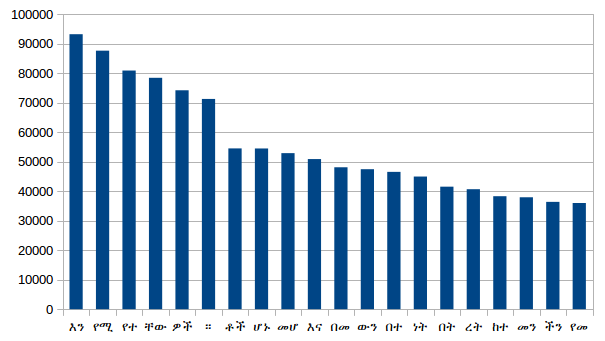
\includegraphics[width=0.5\textwidth]{fig_top20_digraph}
\centering
\end{figure}

\subsection{Trigram frequency}
Just as bigram counts count the frequency of pairs of characters, trigram counts count the frequency of triple characters\cite{text_characterisation}.

\selectlanguage{ethiop}
\begin{table}[H]
    \begin{center}
        \begin{tabular}{|| r | l | r || r | l | r ||}
            \hline
            \foreignlanguage{english}{ } &
            \foreignlanguage{english}{Character} &
            \foreignlanguage{english}{Count} &
            \foreignlanguage{english}{ } &
            \foreignlanguage{english}{Character} &
            \foreignlanguage{english}{Count} \\
            \hline
            \hline
                1 & mahonu & 46465 & 11 & yo.peyA & 16220   \\
                2 & le:: & 25242 & 12 & teyo.pe & 16074     \\
                3 & 'enedi & 25239 & 13 & masara & 15673    \\
                4 & lE:: & 24421 & 14 & bEto^ce & 15665     \\
                5 & 'enedu & 22040 & 15 & 'iteyo & 15617    \\
                6 & 'egezi & 21588 & 16 & hisAbe & 15541    \\
                7 & yamiyA & 20648 & 17 & minise & 15304    \\
                8 & wese^Ce & 18908 & 18 & honune & 14916   \\
                9 & manege & 18554 & 19 & ba^gate & 14504   \\
                10 & ^cawene & 16357 & 20 & 'eneda & 14436  \\
            \hline
        \end{tabular}
    
        \selectlanguage{english}
        \caption{Top 20 - Trigram frequency}
        \label{table:3}
    \end{center}
\end{table}

\selectlanguage{english}
\begin{figure}[H]
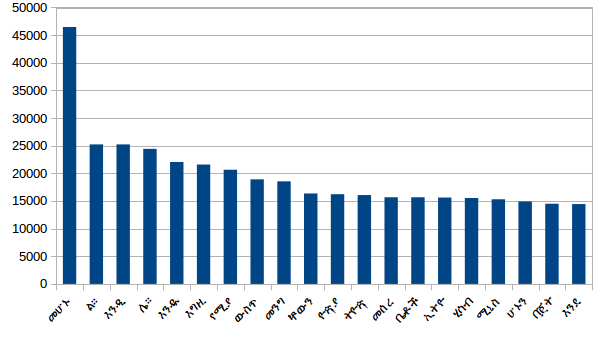
\includegraphics[width=0.5\textwidth]{fig_top20_trigraph}
\centering
\end{figure}

\subsection{Consonant group ('\foreignlanguage{ethiop}{bEte}') frequency}

Consonant group frequency is the frequency of the 34 Amharic consonant variants which is one row from the Ge`ez script consonants cluster. All of the '\foreignlanguage{ethiop}{ha}', '\foreignlanguage{ethiop}{hu}', '\foreignlanguage{ethiop}{hi}', '\foreignlanguage{ethiop}{hA}' ... variants are grouped together and analyzed\cite{ethiopic_scripts}. 

\selectlanguage{ethiop}
\begin{table}[H]
    \begin{center}
        \begin{tabular}{|| r | l | r || r | l | r ||}
        \hline
        \foreignlanguage{english}{ } &
        \foreignlanguage{english}{Character} &
        \foreignlanguage{english}{Count} &
        \foreignlanguage{english}{ } &
        \foreignlanguage{english}{Character} &
        \foreignlanguage{english}{Count} \\
        \hline
        \hline
            1 & ta & 1502138 & 11 & 'a & 698619 \\
            2 & na & 1462331 & 12 & da & 640813 \\
            3 & ya & 1408562 & 13 & ka & 598522 \\
            4 & ma & 1382417 & 14 & ha & 497119 \\
            5 & ba & 1170744 & 15 & ^ca & 408120 \\
            6 & ra & 1131021 & 16 & qa & 386470 \\
            7 & la & 967577 & 17 & ^Ca & 375543 \\
            8 & wa & 844325 & 18 & fa & 277775 \\
            9 & sa & 759615 & 19 & za & 261978 \\
            10 & ga & 736809 & 20 & ^ga & 182281 \\
        \hline
        \end{tabular}
    
        \selectlanguage{english}
        \caption{Consonant group ('\foreignlanguage{ethiop}{bEte}') frequency}
        \label{table:4}
    \end{center}
\end{table}

\begin{figure}[H]
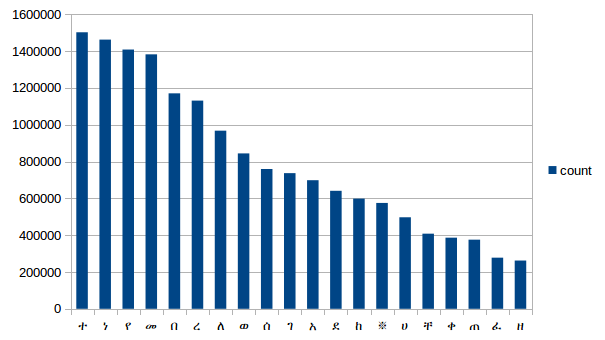
\includegraphics[width=0.48\textwidth]{fig_top20_bet-graph}
\centering
\end{figure}

\begin{figure}[H]
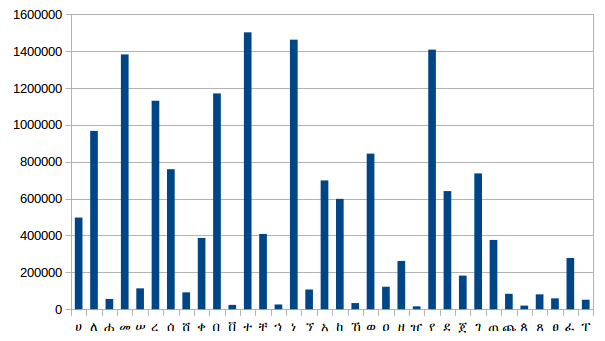
\includegraphics[width=0.48\textwidth]{fig_all_bet-graph}
\centering
\end{figure}

\selectlanguage{english}

\subsection{Vowel group ('\foreignlanguage{ethiop}{madabe}') frequency}
Vowel group frequency is the frequency of the vowel variants which will modify each consonant (i.e one column from the Ge`ez script consonants cluster). All of the '\foreignlanguage{ethiop}{sAdese}' variants ('\foreignlanguage{ethiop}{he}', '\foreignlanguage{ethiop}{le}', '\foreignlanguage{ethiop}{.he}', '\foreignlanguage{ethiop}{me}' ... ) are grouped together and analyzed\cite{ethiopic_scripts}.

\selectlanguage{ethiop}
\begin{table}[H]
    \begin{center}
        \begin{tabular}{|| r | r | l | r ||}
        \hline
        \foreignlanguage{english}{} & 
        \foreignlanguage{english}{Character} & 
        \foreignlanguage{ethiop}{madabe} & 
        \foreignlanguage{english}{Count} \\
        \hline
        \hline
        1 & 6 & \foreignlanguage{ethiop}{sAdese} & 5848229 \\
        2 & 1 & \foreignlanguage{ethiop}{ge`eze} & 4933207 \\
        3 & 4 & \foreignlanguage{ethiop}{rAbe`e} & 2661791 \\
        4 & 2 & \foreignlanguage{ethiop}{kA`ebe} & 1046439 \\
        5 & 3 & \foreignlanguage{ethiop}{'sAlese} & 1044916 \\
        6 & 7 & \foreignlanguage{ethiop}{sAbe`e} & 720252 \\
        7 & 5 & \foreignlanguage{ethiop}{_hAmese} & 680979 \\
        8 & 8 & \foreignlanguage{ethiop}{zamada rAbe`e} & 318991 \\
        \hline
        \end{tabular}
        
        \selectlanguage{english}
        \caption{Top 20 - Vowel group ('\foreignlanguage{ethiop}{madabe}') frequency}
        \label{table:5}
    \end{center}
\end{table}

\selectlanguage{english}
\begin{figure}[H]
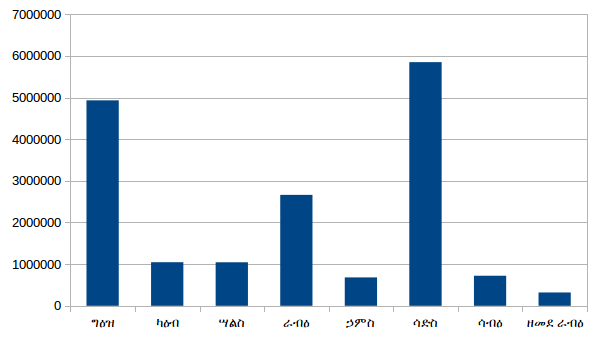
\includegraphics[width=0.48\textwidth]{charts/fig_all_medeb-graph}
\centering
\end{figure}

\subsection{Double letter frequency}
A double-letter word is one that contains consecutive letters that are the same, such as rabbit, deer or kitten. For each letter of the alphabet, this are the most common double letters in Amharic.

\selectlanguage{ethiop}
\begin{table}[H]
    \begin{center}
    \begin{tabular}{|| r | l | r || r | l | r ||}
    \hline
    \foreignlanguage{english}{ } & 
    \foreignlanguage{english}{Character} &
    \foreignlanguage{english}{Count} &
    \foreignlanguage{english}{ } & 
    \foreignlanguage{english}{Character} &
    \foreignlanguage{english}{Count} \\
    \hline
    \hline
    1 & : & 71312 & 11 & me & 3091 \\
    2 & ma & 17992 & 12 & le & 3056 \\
    3 & ^sA & 9540 & 13 & lE & 2362 \\
    4 & te & 8785 & 14 & we & 2031 \\
    5 & ne & 6474 & 15 & nA & 1925 \\
    6 & yA & 6255 & 16 & sA & 1891 \\
    7 & ^Ce & 6024 & 17 & ^CA & 1867 \\
    8 & ke & 5975 & 18 & tA & 1836 \\
    9 & ba & 4090 & 19 & ta & 1701 \\
    10 & qua & 3769 & 20 & lA & 1616 \\
    \hline
    \end{tabular}
    
    \selectlanguage{english}
    \caption{Top 20 - Double letter frequency}
    \label{table:6}
    \end{center}
\end{table}

\selectlanguage{english}
\begin{figure}[H]
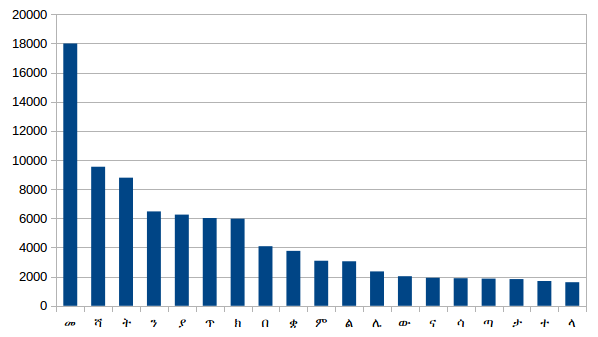
\includegraphics[width=0.48\textwidth]{charts/fig_all_double_letter-graph}
\centering
\end{figure}

\subsection{First letter frequency}
First letter frequency is the frequency of a given Amharic language first letter from a given word. 

\selectlanguage{ethiop}
\begin{table}[H]
    \begin{center}
    \begin{tabular}{|| r | l | r || r | l | r ||}
    \hline
    \foreignlanguage{english}{ } & 
    \foreignlanguage{english}{Character} &
    \foreignlanguage{english}{Count} &
    \foreignlanguage{english}{ } & 
    \foreignlanguage{english}{Character} &
    \foreignlanguage{english}{Count} \\
    \hline
    \hline
    1 & ya & 569324 & 11 & yA & 72231 \\
    2 & ba & 414816 & 12 & la & 71432 \\
    3 & ma & 259743 & 13 & se & 66667 \\
    4 & 'e & 238565 & 14 & ge & 48456 \\
    5 & 'a & 208080 & 15 & we & 42183 \\
    6 & ka & 121484 & 16 & me & 42005 \\
    7 & ta & 117446 & 17 & ke & 41459 \\
    8 & wa & 85590 & 18 & bA & 41416 \\
    9 & mA & 78348 & 19 & be & 40596 \\
    10 & ye & 72597 & 20 & li & 38199 \\
    \hline
    \end{tabular}
    
    \selectlanguage{english}
    \caption{Top 20 - First letter frequency}
    \label{table:7}
    \end{center}
\end{table}

\selectlanguage{english}
\begin{figure}[H]
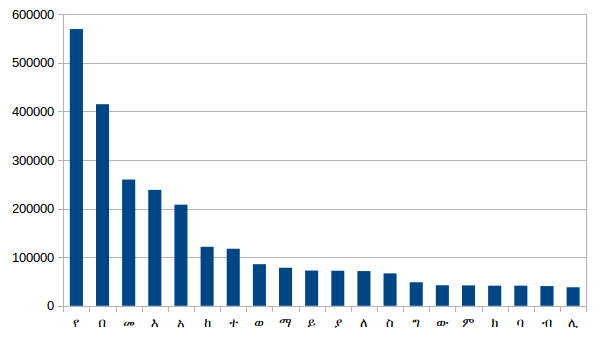
\includegraphics[width=0.48\textwidth]{charts/fig_all_first_letter-graph}
\centering
\end{figure}

\subsection{Second letter frequency}
Second letter frequency is the frequency of a given Amharic language second letter from a given word. 

\selectlanguage{ethiop}
\begin{table}[H]
    \begin{center}
    \begin{tabular}{|| r | l | r || r | l | r ||}
    \hline
    \foreignlanguage{english}{ } & 
    \foreignlanguage{english}{Character} &
    \foreignlanguage{english}{Count} &
    \foreignlanguage{english}{ } & 
    \foreignlanguage{english}{Character} &
    \foreignlanguage{english}{Count} \\
    \hline
    \hline
    1 & ne & 211523 & 11 & nA & 74411 \\
    2 & ma & 171288 & 12 & la & 68440 \\
    3 & ta & 147704 & 13 & ho & 66992 \\
    4 & re & 129813 & 14 & be & 59655 \\
    5 & mi & 124359 & 15 & me & 57804 \\
    6 & se & 113693 & 16 & sa & 53831 \\
    7 & mA & 95597 & 17 & le & 52029 \\
    8 & ye & 93176 & 18 & 'a & 51903 \\
    9 & ga & 82967 & 19 & we & 51116 \\
    10 & ge & 78444 & 20 & rA & 49058 \\
    \hline
    \end{tabular}
    
    \selectlanguage{english}
    \caption{Top 20 - Second letter frequency}
    \label{table:8}
    \end{center}
\end{table}

\selectlanguage{english}
\begin{figure}[H]
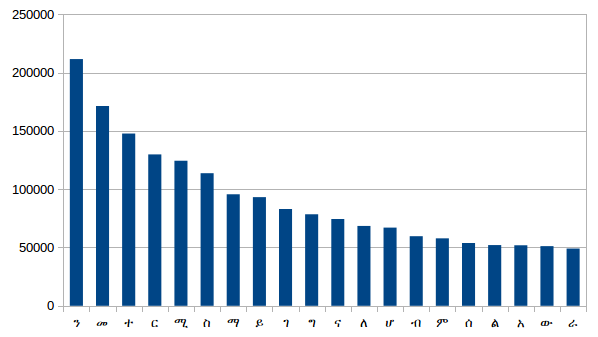
\includegraphics[width=0.48\textwidth]{charts/fig_all_second_letter-graph}
\centering
\end{figure}

\subsection{Last letter frequency}
Last letter frequency is the frequency of a given Amharic language last letter from a given word. 


\selectlanguage{ethiop}
\begin{table}[H]
    \begin{center}
    \begin{tabular}{|| r | l | r || r | l | r ||}
    \hline
    \foreignlanguage{english}{ } & 
    \foreignlanguage{english}{Character} &
    \foreignlanguage{english}{Count} &
    \foreignlanguage{english}{ } & 
    \foreignlanguage{english}{Character} &
    \foreignlanguage{english}{Count} \\
    \hline
    \hline
    1 & te & 467777 & 11 & ye & 75082 \\
    2 & ne & 273331 & 12 & ; & 69485 \\
    3 & nA & 247121 & 13 & be & 65238 \\
    4 & : & 212763 & 14 & le & 64701 \\
    5 & we & 208305 & 15 & tu & 63441 \\
    6 & re & 190347 & 16 & :: & 59351 \\
    7 & ^ce & 156041 & 17 & se & 56831 \\
    8 & me & 138486 & 18 & lE & 51317 \\
    9 & , & 88674 & 19 & rA & 51164 \\
    10 & yA & 82511 & 20 & := & 50495 \\
    \hline
    \end{tabular}
    
    \selectlanguage{english}
    \caption{Top 20 - Last letter frequency}
    \label{table:9}
    \end{center}
\end{table}

\selectlanguage{english}
\begin{figure}[H]
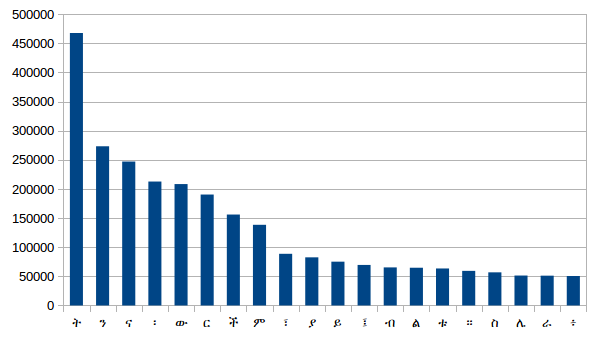
\includegraphics[width=0.48\textwidth]{charts/fig_all_last_letter-graph}
\centering
\end{figure}

\subsection{Word length frequency}
The frequency of the Amharic language words length statistics. 
\begin{table}[H]
    \begin{center}
    \begin{tabular}{|| r | l | r ||}
    \hline
    \foreignlanguage{english}{ } & 
    \foreignlanguage{english}{Length} &
    \foreignlanguage{english}{Count} \\
    \hline
    \hline
    1 & 4 & 928666 \\
    2 & 3 & 787376 \\
    3 & 5 & 701324 \\
    4 & 6 & 437831 \\
    5 & 2 & 367253 \\
    6 & 7 & 170080 \\
    7 & 8 & 69592 \\
    8 & 9 & 21743 \\
    9 & 1 & 16734 \\
    10 & 10 & 5602 \\
    \hline
    \end{tabular}
    
    \selectlanguage{english}
    \caption{Top 20 - Word length frequency}
    \label{table:10}
    \end{center}
\end{table}

\selectlanguage{english}
\begin{figure}[H]
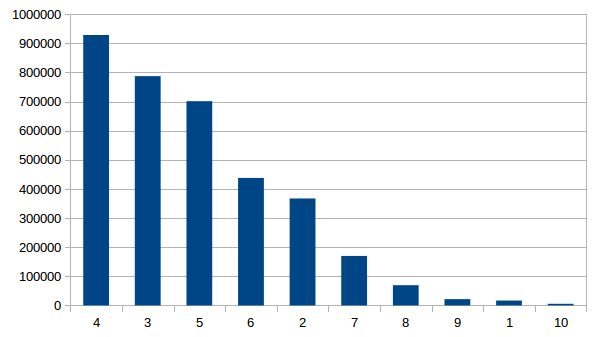
\includegraphics[width=0.48\textwidth]{charts/fig_all_word-length-graph}
\centering
\end{figure}

\section{Discussion}

The Amharic language is the second most spoken  Semitic language and the official language is Ethiopia which the frequency distribution never been analyzed to acquire its frequency distribution. My analysis has uncovered a lot of statistics which will be instrumental in a lot of fields including but not limited to cryptanalysis, linguistics, and optical character recognition. These findings are self-explanatory but I would discuss some observations I found interesting.

I noticed the top 23 frequent monograms occurs more than 50 percent which means the more than half of every Amharic text is composed of only 23 characters.

The decline of the word separator ':' ('\foreignlanguage{ethiop}{hulate na.tebe}') and the use of space like English was also noticeable. Only a few texts I found from religious sites contain texts with the word separator ':'. But still, it's the most frequent punctuation in an Amharic text followed by '\foreignlanguage{ethiop}{,}' (comma),  '\foreignlanguage{ethiop}{;}' (semicolon) and '\foreignlanguage{ethiop}{::}'. Further, I have noticed writers chose to type two consecutive word separator (':') instead of the '\foreignlanguage{ethiop}{::}' full stop (period) which has it's own single glyph in Unicode with (0x1362) code point.

Another statics I noticed was that despite the letter ('\foreignlanguage{ethiop}{ne}') is the most frequent letter,  it's doesn't frequently occur in the first letter of a given word like the letter ('\foreignlanguage{ethiop}{ya}'). On the other hand, 83\% of the letter ('\foreignlanguage{ethiop}{ya}') occurred in the leading (first) position of the word from the total occurrence.

\section{Conclusion}

In conclusion, anyone can use this results to break an Amharic plain text encrypted with cryptographic algorithms which don't adequately hide the language statistical distribution of the letters. These findings should also be used to develop an efficient keyboard layout which is optimized for speed, number of required key combination and hand movements. The results will also be valuable for researchers and experts developing an Amharic optical character recognition software using this data to prioritize and optimize their algorithm to the most frequent letters. They can also predict when challenged using this result. The possibility is innumerable to use this knowledge, I hope it will be useful for all who finds it.
\section{Limitations of the study}

The first limitations I was faced was the lack of a large dataset of processable Amharic text, Which took me more than half of my time doing this analysis. When some texts were found, most of them were just a scanned version of the printed book or newspaper which made it hard for processing.

The lack of publicly available (open source) optical character recognition(OCR) for the Amharic language made it hard to analyze the scanned version of the printed book or newspaper. If OCR was available it was possible to analyze additional datasets which were stored as an image.

One of the analyses I was planning to do was the root word (\foreignlanguage{ethiop}{serewa qAle}) frequency which will give a great insight into the most common words we use in the language. Analysing an Amharic word into their constituent morphemes (meaningful parts) is a challenging by itself and out of this paper scope. So I used 'HORNMORPHO 2.5'\cite{HornMorpho} python package developed by Michael Gasser of Indiana University, School of Informatics and Computing.  HORNMORPHO is a Python program that analyzes Amharic, Oromo, and Tigrinya words into their constituent morphemes (meaningful parts) and generates words, given a root or stem and a representation of the word’s grammatical structure. HORNMORPHO is very slow and requires a high computational capability to analyze millions of words. So, I have excluded root word frequency from this paper.

I also have faced another limitation when I conduct the word length frequency. I have stated in the methodology section, I have used 'pdftotext' conversion tool to convert the documents to a plain file. In some of the texts, I have noticed the tool was not recognizing the space between words and it was combined them into a single word. For example, I have found 50 character length word '\foreignlanguage{ethiop}{gamegAmibAlamuyAwo^cegArekamaqerabA^cawubafitebaqedemiyAsefalAgiwuhulu}' which is understandable and can be divided into a properly separated words '\foreignlanguage{ethiop}{gamegAmi bAlamuyAwo^ce gAre kamaqerabA^cawu bafite baqedemiyA sefalAgiwu hulu}' manually with ease but hard to automate and integrate into the analysis process. Thus I have removed the larger word length occurrences.

Lastly, I want to point out that more than 50 percent of the text I found was religiously or politically biased. Most of the available processable text out there is biased which made my trigram frequency to not look native. 
\section{Recommendations}

I want to urge researchers in the relevant scientific community with a bigger dataset to use the tools I developed, to analyze for better quality results. Whom that with a large computational power use HORNMORPHO\cite{HornMorpho} package to investigate the root word frequency which holds a valuable statistics.

\section{Acknowledgements}

I would like to thank Ermias, Tariku, and Mulat from crypto analysis team for advising, reviewing, and supporting me write this paper. Special thanks for Yilikal Argaw for his support to gather a lot of publicly available Amharic documents.


\section{Appendex}
The software I developed with the full result is available at \url{https://github.com/SamAsEnd/amharic-letter-frequency-distribution}.

\printbibliography

\end{document}
